\begin{frame}{The Stern--Gerlach experiment}
\begin{columns}[c]
\column{0.52\textwidth}
Shoot silver atoms through a magnetic field along the `up-down' ($Z$) direction

\bigskip Naively, one expects a smeared-out distribution

\uncover<5->
{\bigskip
In fact \emph{two} beams, $\spinup$ or $\spindown$: \emph{quantised}}

\uncover<6->
{\bigskip
Rotate the magnets to the `left-right' ($X$) direction: again two beams}

\uncover<7->
{\bigskip
We could naively think that the atom carries predetermined outcomes for $X$ and $Z$ measurements}
\column{0.45\textwidth}
\centering
\only<1>{\sterngerlach{0}}%
\only<2>{\sterngerlach{1}}%
\only<3>{\sterngerlach{2}}%
\only<4>{\sterngerlach{3}}%
\only<5->{\sterngerlach{4}}
\end{columns}
\end{frame}


% ---------------------------------------------------------------------------
\begin{frame}{A more complex experiment}
\centering
\uncover<1->{Keep only $\spinup$ after an `up-down' ($Z$) Stern-Gerlach experiment}

\medskip
\uncover<2->{Measure along $X$: $50\%$ $\spinright$ and $50\%$ $\spinleft$}

\medskip
\uncover<3->{Keep only $\spinright$}

\medskip
\uncover<4->{Measure along $Z$ again: once more $50\%$ $\spinup$ and $50\%$ $\spindown$}

\bigskip
\only<1>{\sgsequence{1}}%
\only<2>{\sgsequence{2}}%
\only<3>{\sgsequence{3}}%
\only<4->{\sgsequence{4}}

\bigskip
\uncover<5->{%
\alt<6->{%
$|{\spinright}\ra = \tfrac{1}{\sqrt{2}}\,|{\spinup}\ra + \tfrac{1}{\sqrt{2}}\,|{\spindown}\ra$ is a \emph{superposition},

\medskip
but so is $|{\spinup}\ra = \tfrac{1}{\sqrt{2}}\,|{\spinleft}\ra + \tfrac{1}{\sqrt{2}}\,|{\spinright}\ra$%
}{%
$\spinright = (50\%)\ \spinup + (50\%)\ \spindown\vphantom{\tfrac{1}{\sqrt{2}}}$ is a \emph{superposition},

\medskip
but so is $\spinup = (50\%)\ \spinleft + (50\%)\ \spinright\vphantom{\tfrac{1}{\sqrt{2}}}$%
}}
\end{frame}


% ---------------------------------------------------------------------------
\begin{frame}{Superposition of two water waves}
\begin{columns}[c]
\column{0.52\textwidth}
Two waves add up: they reinforce or cancel each other

\bigskip
This is called \emph{interference}

\bigskip
The quantum wave: $|\psi\ra = a\,|{\spinup}\ra + b\,|{\spindown}\ra$
\column{0.45\textwidth}
\centering
\only<1>{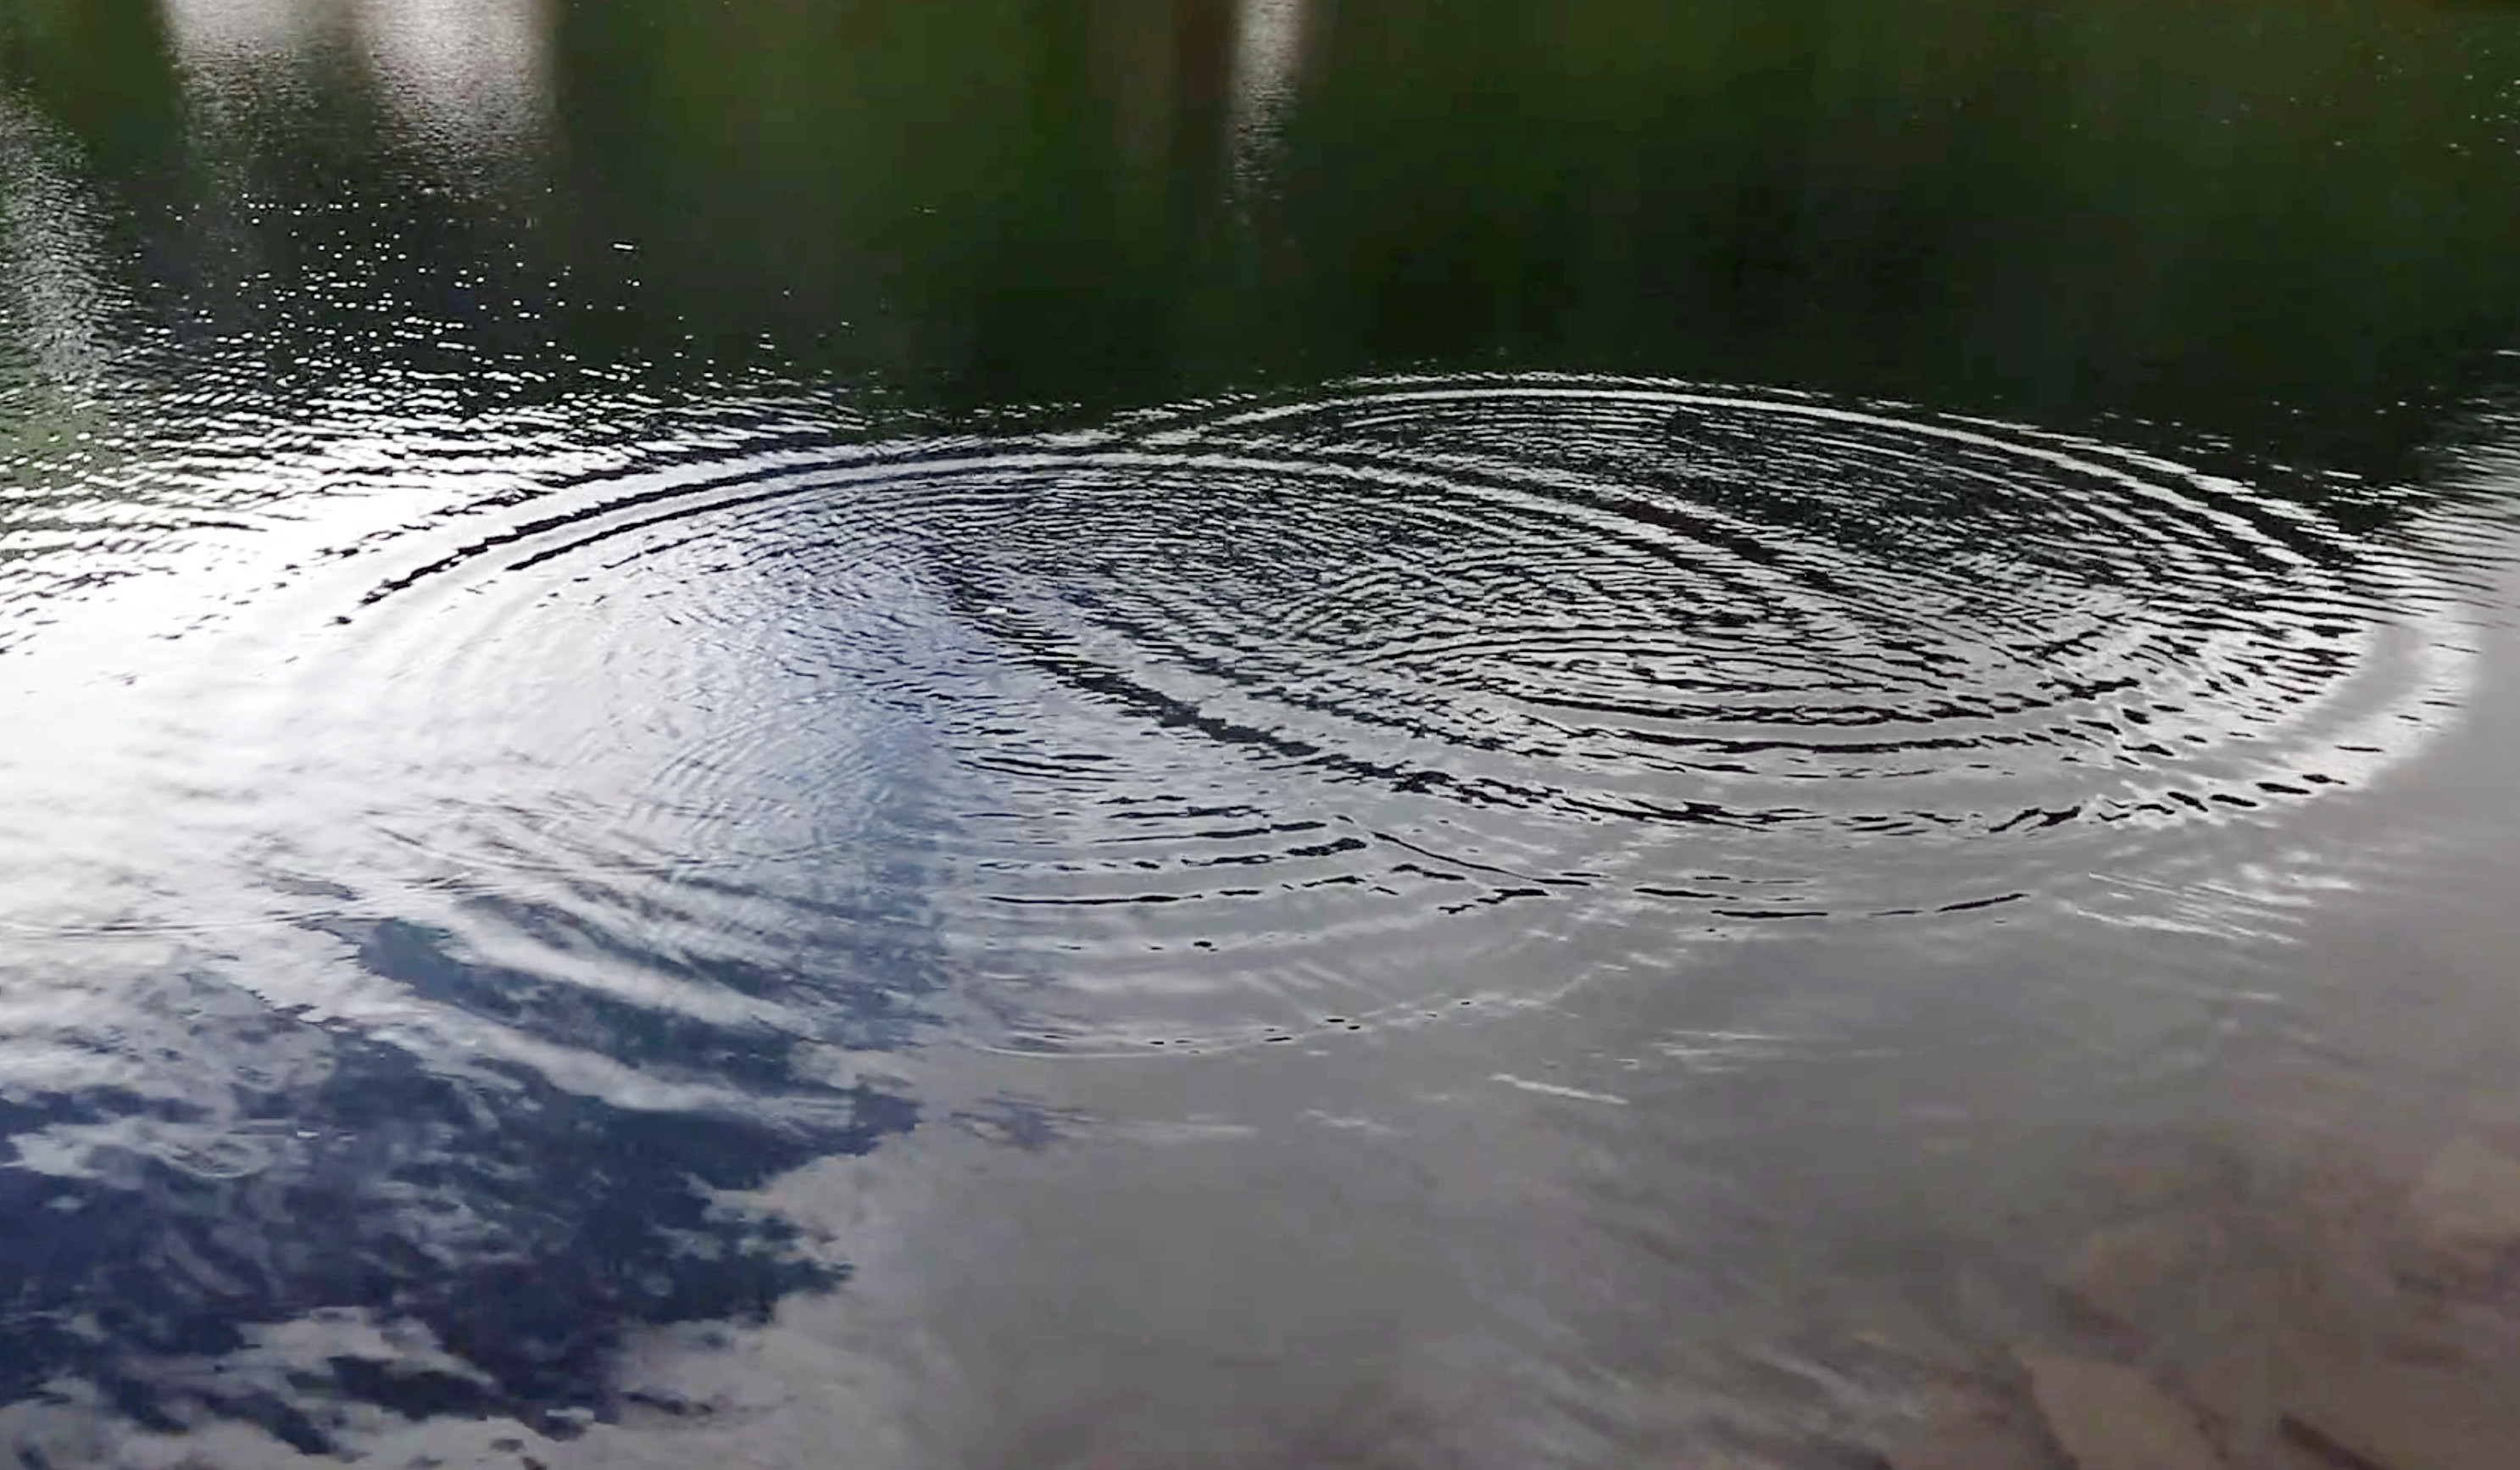
\includegraphics[width=0.85\textwidth]{figs/water_waves.jpg}}
\only<2>{\WaterWaves}
\end{columns}
\end{frame}

% % ---------------------------------------------------------------------------
% \begin{frame}{De Broglie: small and/or cold}
% \begin{columns}[c]
% \column{0.52\textwidth}
% To every particle there is an associated wavelength $\lambda_\text{th} = \frac{1}{\sqrt{2\pi {\color{UGentBlue}m T}}}$

% \bigskip
% This wave behaviour becomes visible when particles are \emph{small} and/or \emph{cold}
% \column{0.45\textwidth}
% \centering
% 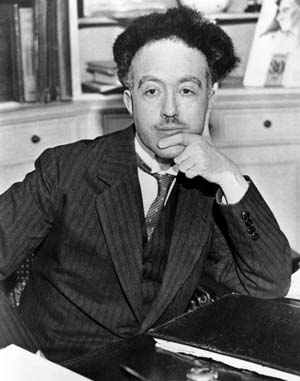
\includegraphics[width=.6\linewidth]{figs/DeBroglie.jpg}
% \end{columns}
% \end{frame}


% ---------------------------------------------------------------------------
\begin{frame}{Many particles}
\begin{columns}[c]
\column{0.52\textwidth}
Recall: together, particles show interesting behaviour, such as magnetism

\bigskip
What does superposition do when there is more than one particle?
\column{0.45\textwidth}
\centering
\fbox{\parbox[c][4cm][c]{0.9\linewidth}{\centering Figure: lattice of spins\\ (from part 1)}}
\end{columns}
\end{frame}


% ---------------------------------------------------------------------------
\begin{frame}{Two particles}
\centering
2 particles: four possibilities: $|{\spinup\spinup}\ra$, $|{\spinup\spindown}\ra$, $|{\spindown\spinup}\ra$, $|{\spindown\spindown}\ra$

\bigskip
Quantum physics dictates: any superposition should be considered:
\[
  |\psi\ra = a\,|{\spinup\spinup}\ra + b\,|{\spinup\spindown}\ra + c\,|{\spindown\spinup}\ra + d\,|{\spindown\spindown}\ra
\]

\bigskip
Let us consider the state
\[
\entangledpair{0} = \tfrac{1}{\sqrt{2}}\big(|{\spinup\spinup}\ra + |{\spindown\spindown}\ra\big)
\]

\end{frame}


% % ---------------------------------------------------------------------------
% \begin{frame}{Mathematics and computer simulations}
% \centering
% A state is a list of numbers $a, b, c, d, \ldots$

% \bigskip
% This mathematics allows for computer simulations

% \bigskip
% The real problem: \emph{finding} the right numbers
% \end{frame}


% % ---------------------------------------------------------------------------
% \begin{frame}{Entanglement}
% \centering
% $\tfrac{1}{\sqrt{2}}\big(|{\spinup\spinup}\ra + |{\spindown\spindown}\ra\big)$: perfectly correlated

% \bigskip
% $\tfrac{1}{\sqrt{2}}\big(|{\spinup\spindown}\ra + |{\spindown\spinup}\ra\big)$: perfectly anti-correlated

% \bigskip
% Each particle separately: $50/50$, yet together always parallel, or always antiparallel

% \bigskip
% \fbox{\parbox[c][2.5cm][c]{0.8\textwidth}{\centering Figure: two entangled spins, measured far apart}}
% \end{frame}


% ---------------------------------------------------------------------------
\begin{frame}{The whole is more than the sum of its parts}
\begin{columns}[c]
\column{0.52\textwidth}
An entangled state cannot be described particle by particle

\bigskip
{\it [...] the best possible knowledge of a whole does not necessarily include the best possible knowledge of all its part [...]}

\smallskip
{\scriptsize E.~Schr\"odinger (1935)}

\column{0.45\textwidth}
\centering
\only<1>{\entangledoutcomes{0}}%
\only<2>{\entangledoutcomes{1}}%
\only<3>{\entangledoutcomes{2}}
\end{columns}
\end{frame}